\documentclass[10pt, compress]{beamer}  
\usetheme{metropolis}
%\usepackage{setspace} %this broke footnotes
\usepackage{epstopdf,amsmath,amsfonts,amssymb,amsthm}
\usepackage{jf}
\usepackage{hyperref}
%\usepackage[margin=1.0in]{geometry}
%\usepackage{placeins}
\usepackage{rotating}
%\usepackage[utf8]{inputenc}
\usepackage{booktabs}
\usepackage{pifont}
%\usepackage{tikz}
\usepackage{pgfplots}
\usepgfplotslibrary{dateplot}
\usepackage{tikzscale}
\usepgfplotslibrary{fillbetween}
%\usepackage[flushleft]{threeparttable}

\usepackage[most]{tcolorbox}% http://ctan.org/pkg/tcolorbox           
\usepackage[normalem]{ulem}                
\usepackage[scale=2]{ccicons}                 
\usepackage[super]{nth}                 
\usepackage{lmodern}
\newcommand{\semitransp}[2][35]{\color{fg!#1}#2}

%\usepackage{natbib}
%\bibliographystyle{jf}  
\usepackage[natbib, authordate, strict, backend=bibtex8, doi=only]{biblatex-chicago}
\addbibresource{sub/capacitybib.bib}
\usepackage{graphicx}
\usepackage[labelfont=bf,labelsep=period]{caption}   % Format figure 
\captionsetup[table]{labelsep=none}

\graphicspath{{.}{./sub/fig}}

%%%%%%%%Uncomment if making printable version for standout correction%%%%%%%
%\setbeamercolor{palette primary}{fg=black, bg=white}

\renewcommand\textbullet{\ensuremath{\bullet}}                  
\setbeamertemplate{bibliography item}{}           


\newcommand{\ctabtitle}[1]{\caption[#1]{\\ \textbf{#1}}}
\newcommand{\ctabsubtitle}[1]{\caption[#1]{\; \textit{#1}}}
\newcommand{\ctabnote}[1]{\begin{flushleft} #1 \end{flushleft}}

\newcommand{\cfigcaption}[2]{\caption[#1]{\textbf{\\#1} \\ #2}}
\newcommand{\cfigtitle}[1]{\caption[#1]{ \\ \textbf{#1} }}
\newcommand{\cfigbeamcaption}[1]{\caption*{\\ #1}}

%Chernov Method
%1) What is the problem?
%2) WHy is it important?
%3) How are you solving the problem?
%4) Results

%%%%%%%%%%%%%Kicker boxes
\definecolor{zaffre}{rgb}{0.0, 0.08, 0.66}
\newtcolorbox{kicker}{colback=zaffre,arc=0.5mm,coltext=white, fontupper=\bfseries, colframe=black, halign=flush left, left=0.75mm, top=0.75mm, bottom=0.75mm, right=0.75mm}

\definecolor{mgrey}{rgb}{0.2824,0.3176,0.298}
\definecolor{lgrey}{rgb}{.7176, .7451, .7333}
\definecolor{vlgrey}{rgb}{.9098, .9176, .9137}
\newtcolorbox{quotebox}[1]{colback=vlgrey,
colframe=mgrey,fonttitle=\bfseries,
title=#1, left=1mm, top=1mm, bottom=1mm, right=1mm}
%%%%%%%%%%%%%%%%%%%%%%%
%Variable fonts per slide
%https://tex.stackexchange.com/questions/33969/changing-font-size-of-selected-slides-in-beamer
\usepackage{environ}
\usepackage{lipsum}

%
% Custom font for a frame.
%
\newcommand{\customframefont}[1]{
\setbeamertemplate{itemize/enumerate body begin}{#1}
\setbeamertemplate{itemize/enumerate subbody begin}{#1}
}

\NewEnviron{framefont}[1]{
\customframefont{#1} % for itemize/enumerate
{#1 % For the text outside itemize/enumerate
\BODY
}
\customframefont{\normalsize}
}

\setbeamercolor{background canvas}{bg=white}
%%%%%%%%%%%%%%%%%%%%%%%%%%%%%


%Some stuff from a previous document, not totallly sure what this is
\setbeamertemplate{blocks}[rounded][shadow=true]                  
\metroset{block=fill}                 
\definecolor{mycolor}{rgb}{0.122, 0.435, 0.698}% Rule colour
\makeatletter


\makeatother
%\author[Tepper]{Clinton Tepper\inst{\text{\ding{169}}}}
%\institute[]{\inst{\text{\ding{169}}} UCLA Anderson School of Management}
\author[Tepper]{iCapital Portfolio Analytics}
\title{\Large \bf GMAM 3.0}

\date{\today}

\begin{document}

\newcommand{\tstar}{\ensuremath{^\text{***}}}
\newcommand{\dstar}{\ensuremath{^\text{**}}}
\newcommand{\ostar}{\ensuremath{^\text{*}}}
\maketitle

%%%%%%%%%%%%%%%%%%%%%%%%%%%%%%%%%%%


%\begin{frame}[fragile]
%\frametitle{The Research Process}
%\begin{figure}
%	\centering
%	%\includegraphics[width=0.95\linewidth]{sub/fig/paxsectionalverification-mfs.pdf}
	%\includegraphics[width=0.95\linewidth]{sub/fig/xmomassetsfs.tikz}
%	\includegraphics[width=1.04\linewidth]{docs/theory/Model Development.pdf}\\
%    \bigskip
%\end{figure}

%\end{frame}

\begin{frame}[fragile]
\frametitle{Full-information models} \label{fr:motivation}
\begin{itemize}
    \item Reduced form models such as those used in GMAM1/2 are parismonious and flexible, but also inefficient and limited in the insights they provide.
    \item []
    \item A comprehensive model of the data-generating process formally represents our understanding of how the asset generates returns.
    \item []
    \item Estimating such a statistical model efficiently uses the data to answer the most pertinent questions about the way a fund generates returns.
    \item []
    \item These models require more advanced statistical techniques such as Maximum Likelihood or Bayesian methods.
\end{itemize}
\end{frame}

\begin{frame}[fragile]
\frametitle{A Bayesian Model: Motivation} \label{fr:motivation}
\begin{itemize}
    \item Frequentist methods fix the parameters in the data-generating process (DGP) and assume the data is generated randomly. (Maximimum likelihood is frequentist.)
    \item []
    \item Bayesian methods invert the DGP by fixing the data and inferring the likely distribution of parameters.
    \item []
    \item Bayesian estimators are admissible in the statistical sense: given the data generating process and a loss function, no other estimator always performs better (weakly dominates) the Bayesian estimator.
    \item []
    \item Drawbacks: priors (sometimes), tractability, and performance.
\end{itemize}
\end{frame}

\begin{frame}[fragile]
\frametitle{A Bayesian Model: Motivation} 
\begin{itemize}
    \item Priors influence the results, but they also serve as a convenient and statistically rigorous approach for incorporating outside information (e.g. cross-sectional data) into the estimates.
    \item []
    \item Tractability issues stem from what is also Bayesian model's greatest strength: every unknown parameter is viewed probabilistically with respect to the values it can take given fixed observations.
    \item []
    \item Performance issues are specific to the solution methodology, but the most common (MCMC) requires extensive simulation in the estimation process. GMAM 3 is no different, but the MCMC approach is highly scalable and amenable to a cacheing architecture.
    
    \item []
    \vspace{12pt}
    \begin{kicker}
        The GMAM 3 model delivers the advantages of a Bayesian approach while staying feasible to implement and estimate.
    \end{kicker}
\end{itemize}
\end{frame}


\begin{frame}[fragile]
\frametitle{Bayesian Estimation}
\begin{itemize}
    \item Suppose a set of data $y$ is normally distributed.
    \item []
    \item The econometrician seeks to estimate the likely range for the mean and variance distributed with density $p(\mu,\sigma^2|y)$.
    \item []
    \item By Bayes theorem:
    \begin{align*}
        p(\mu,\sigma^2|y) &= \frac{p(y|\mu,\sigma^2) \times p(\mu) \times p(\sigma^2)}{p(y)}\\
        &\propto p(y|\mu,\sigma^2) \times p(\mu) \times p(\sigma^2)
    \end{align*}
    The second line follows from the Bayesian's interpretation of the observations as fixed.
    \item[]
    \item Bayesian approaches harness the property that the parameters $\mu$ and $\sigma^2$ are distributed with density proportional to the likelihood given the parameters times the parameter priors.
\end{itemize}
\end{frame}

\begin{frame}[fragile]
\frametitle{MCMC}
\begin{itemize}
    \item Markov Chain Monte Carlo (MCMC) is a highly flexible procedure for computing the distribution of parameter estimates given the data.
    \item []
    \item In infinite time and mild regularity conditions, MCMC provides the EXACT distribution of the posterior.
\end{itemize}
\end{frame}

\begin{frame}[fragile]
\frametitle{Bayesian Estimation: MCMC}
\begin{itemize}
    \item For the previous example, the MCMC is implemented as follows:
    \begin{align}
        \mu_i &\sim p\left(\mu | \sigma^2_{i-1},D\right)\\
        \sigma^2_i &\sim p\left(\sigma^2 | \mu_i,D\right)
    \end{align}
    \item In the long-run, the parameters drawn in this manner are distributed in accordance with their marginal posterior distributions.
\end{itemize}
\end{frame}


\begin{frame}[fragile]
\frametitle{Mean Field Variational Bayes: Application to GMAM 3.0}

In GMAM 3, the parameters (collectively $\Theta$) are constrained by observations fund returns $y$ and factor returns $F$:
\begin{align*}
    p\left(\Theta|rest\right)& \propto p(y|rest)\times p\left(x|\beta,\phi,\tau_{x},\tau_{y},\psi,F\right)\\
    &\times p\left(\phi|\tau_{y},\tau_{\phi}\right)\times p\left(\beta|\gamma,\tau_{x},\tau_{y},\tau_{\beta}\right)\times p\left(\gamma|\omega\right)\times p\left(\omega\right)\\
    &\times p\left(\psi|\nu\right)\times p\left(\nu\right)\times p\left(\tau_{x}\right)\times p\left(\tau_{y}\right)\times p\left(\tau_{\phi}\right)\times p\left(\tau_{\beta}\right)
\end{align*}

\begin{table}
\scriptsize

%\caption{\bf\scriptsize \;Explanatory volume regressions (1 month, 18-month rolling)}
\vspace{-10pt}   
    \begin{tabular}{ccl}
    \toprule 
        Variable & Type & Definition/Description\tabularnewline
        \midrule
            $x$ & Local & $x$ is a vector of latent economic returns\tabularnewline
            $\phi$ & Local & $\phi$ is the moving average window\tabularnewline
            $\tau_{y}$ & Global & Precision parameter for independent measurement error\tabularnewline
            $\tau_\phi$ & Global & Precision parameter for prior on $\phi$\tabularnewline
            $\beta$ & Local & Regression coefficients of $x$ on $F$\tabularnewline
            $\psi$ & Local & $\psi$ is a vector of precision weights for $x$\tabularnewline
            $\tau_{x}$ & Global & Precision parameter for the regression of $x$ on $F$\tabularnewline
            $\gamma$ & Local & Vector of variable selection indicators\tabularnewline
            $\omega$ & Global & Probability of variable selection\tabularnewline
            $\nu$ & Global & DOF of the $x$ conditional posterior $t$ distribution\tabularnewline
            $\tau_\beta$ & Global & Precision parameter for prior on $\beta$\tabularnewline
            
        \bottomrule
    \end{tabular}
\end{table}
\end{frame}

\begin{frame}[fragile]
\frametitle{GMAM 3.0}
\begin{figure}
	\centering
	%\includegraphics[width=0.95\linewidth]{sub/fig/paxsectionalverification-mfs.pdf}
	%\includegraphics[width=0.95\linewidth]{sub/fig/xmomassetsfs.tikz}
	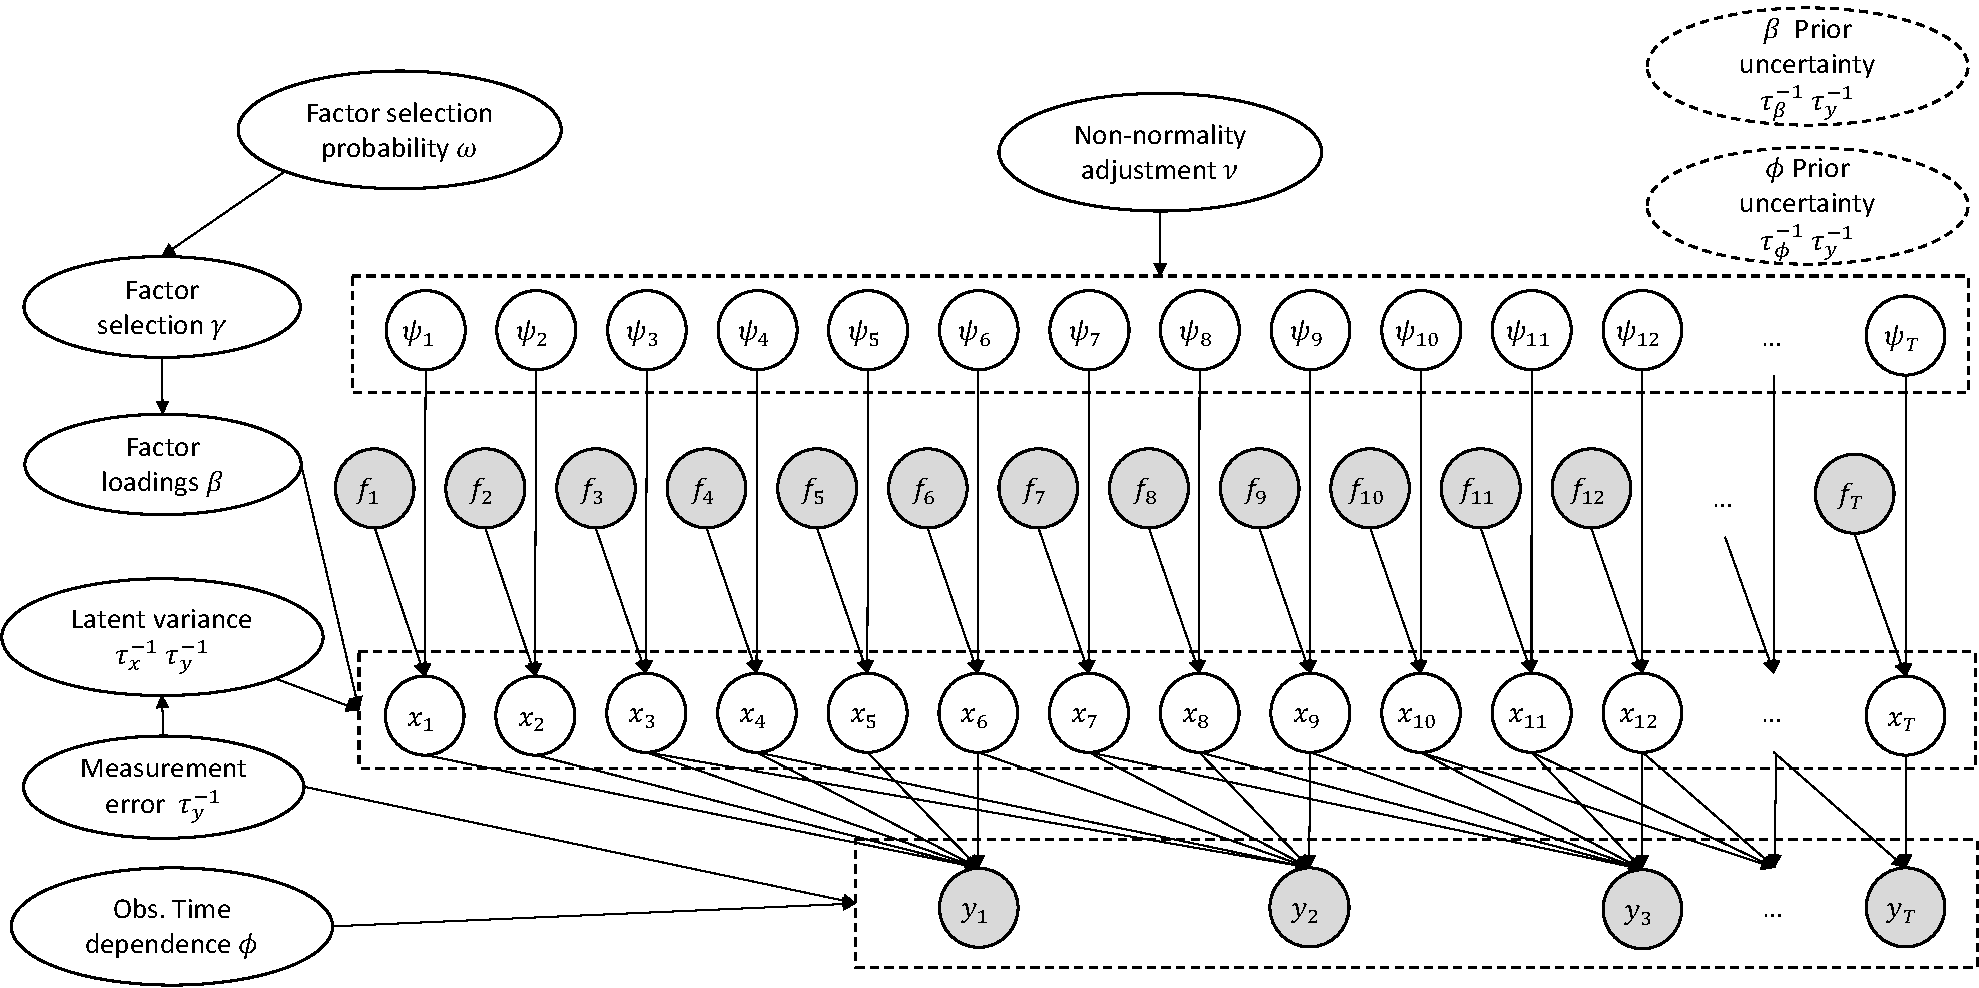
\includegraphics[width=1.04\linewidth]{docs/theory/DAG.pdf}\\
    \bigskip
    \begin{kicker}
        The hierarchical structure of GMAM 3.0 provides a flexible and rigorous statistical framework for advanced portfolio analytics.
    \end{kicker}
\end{figure}

\end{frame}




\begin{frame}[fragile]
\frametitle{GMAM 3.0: Implementation}
\begin{itemize}
    \item Running GMAM 3.0 on a set of returns consists of the following steps:
    \item []
    \begin{enumerate}
        \item Load the prior hyperparameters
        \item Set initial values for the nine conditional posterior distributions 
        \item Sequentially draw from each of the nine posterior distributions many times.
        \item Drop the burn-in period from the sequence.
        \item Compute all relevant summary stats and analytics from the sequence. Cache the the results if desired.
    \end{enumerate}
\end{itemize}
\end{frame}

\begin{frame}[fragile]
\frametitle{GMAM 3.0: Performance}
\begin{itemize}
    \item On a fast computer, a single chain should converge in a couple minutes.
    \item []
    \begin{itemize}
        \item The estimates better approximate the true posterior as the number of iterations increases.
        \item []
        \item This provides flexibility: longer runs can occur overnight, with shorter passes possible for rough "online" estimates.
        \item []
        \item The research POC includes implementations of numerous diagnostic tools to quantitatively and qualitatively assess convergence.
    \end{itemize}
    \item []
    \item While it is not generally feasible to parallelize the MCMC for a particular fund, each fund estimation can be dropped into its own process.
\end{itemize}
\end{frame}

\begin{frame}[fragile]
\frametitle{GMAM 3.0: Implementation Resources}
\begin{itemize}
    \item The internal model doc contains all of the posterior specifications.
    \begin{itemize}
        \item Probably worth walking through in a separate meeting.    
        \item Derivations are provided. For Alpha, ignore anything in the doc related to the VB approximation method. I will create a clean "Alpha only" version in the near term if we choose to proceed.
    \end{itemize}
    \item []
    \item A research POC provides implementation guidance.
    \begin{itemize}
        \item An important check: Verify that the POC and production variants produce the same results.
    \end{itemize}
    \item []
    \item Please reach out with questions. 
    \begin{itemize}
        \item For now, Aniket has the most familiarity with the model doc outside of myself- both of us are available to help.
    \end{itemize}
\end{itemize}
\end{frame}

\begin{frame}[fragile]
\frametitle{GMAM 3.0 Alpha vs Prime}
\begin{enumerate}
    \item The Alpha version of GMAM 3.0 uses weakly informative priors. 
    \item []
    \item Prime will use the cross-section of data and, in the case of PE funds, previous fund returns to generate more informative priors.
    \item []
    \item Prime should have greater efficacy for new fund launches and limited track records.
    \item []
    \item We expect that the weakly informative priors of GMAM 3 Alpha still provide significantly better regularization and control relative to GMAM 2/1.
\end{enumerate}
\end{frame}

\end{document}